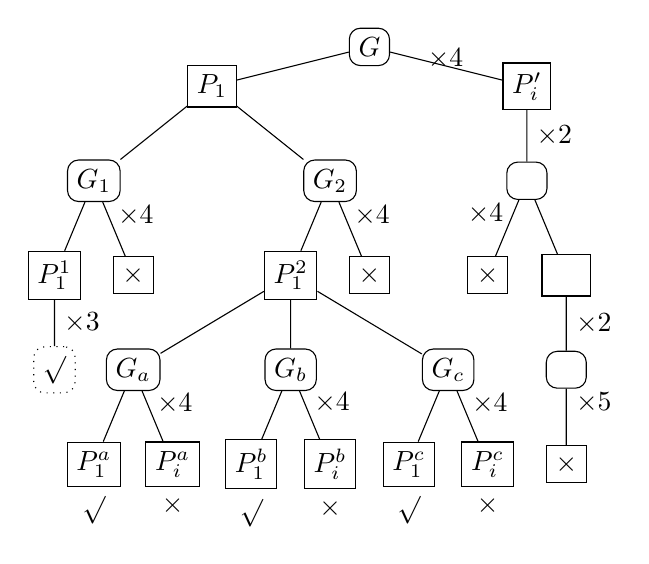
\begin{tikzpicture}[level distance=1.2cm]

\tikzstyle{planbox}=[draw]
\tikzstyle{goalbox}=[draw,rounded corners]

\tikzstyle{level 1}=[sibling distance=4cm,level distance=0.5cm] 
\tikzstyle{level 2}=[sibling distance=3cm,level distance=1.2cm] 
\tikzstyle{level 3}=[sibling distance=1cm]
\tikzstyle{level 4}=[sibling distance=2cm]
\tikzstyle{level 5}=[sibling distance=1cm]

\node[goalbox,yshift=1cm,solid] (T) {$G$}
   child[solid] {node[planbox] (1) {$P_1$}
      child {node[goalbox] {$G_{1}$}
		child {node[planbox] {$P_{1}^1$}
			child {node[goalbox,dotted] {$\surd$}
% 				child {node[planbox,label=below:$\surd$] {$P_{a}^1$}}
% 				child {node[planbox,label=below:$\times$] {$P_{b}^k$}
% 					edge from parent node[right,near start] {$\times 4$}
% 				}
			edge from parent node[right] {$\times 3$}
			}
		}
		child {node[planbox] {$\times$}
			edge from parent node[right,near start] {$\times 4$}
	}
	}
%
      child {node[goalbox] {$G_{2}$}
		child {node[planbox] {$P_{1}^2$}
			child {node[goalbox] {$G_a$}
				child {node[planbox,label=below:$\surd$] {$P_1^a$}}
				child {node[planbox,label=below:$\times$] {$P_i^a$}
					edge from parent node[right,near start] {$\times 4$}
				}
			}
			child {node[goalbox] {$G_b$}
				child {node[planbox,label=below:$\surd$] {$P_1^b$}}
				child {node[planbox,label=below:$\times$] {$P_i^b$}
					edge from parent node[right,near start] {$\times 4$}
				}
			}
			child {node[goalbox] {$G_c$}
				child {node[planbox,label=below:$\surd$] {$P_{1}^c$}}
				child {node[planbox,label=below:$\times$] {$P_i^c$}
					edge from parent node[right,near start] {$\times 4$}
				}
			}
		}
		child {node[planbox] {$\times$}
			edge from parent node[right,near start] {$\times 4$}
	}
	}
      }
%
%
%
%
%
      child[solid] {node[planbox] (1) {$P'_i$}
      child {node[goalbox] {\phantom{$G$}}
		child {node[planbox] {$\times$}
			edge from parent node[left,near start] {$\times 4$}
		}
		child {node[planbox] {\phantom{$P_2$}}
			child {node[goalbox] {\phantom{$\times$}}
				child {node[planbox] {$\times$}
					edge from parent node[right,near start] {$\times 5$}
				}
			edge from parent node[right] {$\times 2$}
			}
		}
	edge from parent node[right] {$\times 2$}
	}
	edge from parent node[right,near start] {$\times 4$}
      };
\end{tikzpicture}

% \begin{tikzpicture}[level distance=1.2cm]
% 
% \tikzstyle{planbox}=[draw]
% \tikzstyle{goalbox}=[draw,rounded corners]
% 
% \tikzstyle{level 2}=[sibling distance=2.8cm] 
% \tikzstyle{level 3}=[sibling distance=3.4cm]
% \tikzstyle{level 4}=[sibling distance=1.8cm]
% \tikzstyle{level 5}=[sibling distance=1cm]
% 
% \node[goalbox,dashed] (G) {$G$}
% child[dashed] { node[planbox,dashed] (top) {$P$}
% child[dashed] {node[goalbox,below left of=top,yshift=1cm,solid] (T) {$G_0$}
%    child[solid] {node[planbox,label=below:$\longrightarrow$] (1) {$P_1$}
%       child {node[goalbox] (11) {$G_{1}$}
% 		child {node[planbox] {$P_3$}}
% 		child {node[planbox] {$P_4$}}
% 	}
%       child {node[goalbox] (12) {$G_{2}$}
% 		child {node[planbox] {$P_5$}}
% 		child {node[planbox] {$P_6$}}
% 	}
%       child {node[goalbox] (13) {$G_{3}$}
% 		child {node[planbox] {$P_7$}}
% 	}
%       }
%    child[solid] {node[planbox] (2) {$P_2$}
%       child {node[goalbox] (22) {$G_{3}$}
% 	child {node[planbox] {$P_8$}}
% 	child {node[planbox] {$P_9$}}
% 	}
%    }
% }
% };
% 
% \draw (T) -- (1) node (aux1) [coordinate,midway]{};
% \draw (T) -- (2) node (aux2) [coordinate,midway]{};
% \draw (aux1) .. controls +(0.3,-0.3) and +(-0.3,-0.3).. (aux2)
% 			node[midway,above] {OR};
% 
% % \draw (1) -- (11) node (aux21) [coordinate,midway]{};
% % \draw (1) -- (12) node (aux23) [coordinate,midway]{};
% % \draw (aux21) .. controls +(0.25,-0.25) and +(-0.25,-0.25).. (aux23)
% % 			node[midway,above] {AND};
% 
% % \node[below left of=T,text width=2cm,xshift=-3cm] (label)
% % 		{$P_i$: plan \\ $G_i$: goals \\ $SG_i$: sub-goals};
% \end{tikzpicture}
